\section{Additional Experimental Details}
\label{app:details}

\para{LoRA target modules.} For Qwen2.5 we adapt \texttt{q\_proj}, \texttt{k\_proj}, \texttt{v\_proj}, \texttt{o\_proj}, \texttt{gate\_proj}, \texttt{up\_proj}, and \texttt{down\_proj}. For Pythia we adapt \texttt{query\_key\_value}, \texttt{dense}, \texttt{dense\_h\_to\_4h}, and \texttt{dense\_4h\_to\_h}.

\para{Memory.} To fit training into 2--5\,GB GPU slices, the loss is computed over 256-token chunks with recomputation, together with gradient checkpointing.

\para{Corpora.} Each run uses a seeded prefix of $\sim$6.1M tokens from its corpus. Code files are 800--20k characters long and filtered to exclude auto-generated files.

\para{Held-out in-domain NLL (nats per token, step 0 $\rightarrow$ step 3,000).}

\begin{table}[h]
    \centering
    \small
    \caption{Held-out in-domain NLL before and after fine-tuning under the standard recipe. Code fine-tuning gives no gain for \qwenS, and \pythiaS LoRA diverges in both domains.}
    \label{tab:nll}
    \begin{tabular}{@{}lcc@{}}
        \toprule
        \textbf{Model} & \textbf{Code} & \textbf{Medical} \\
        \midrule
        \qwenS (lr 2e-4) & 1.58 $\rightarrow$ 1.68 (no gain) & 2.34 $\rightarrow$ {\bf 1.98} (learned) \\
        \pythiaM & 1.55 $\rightarrow$ 1.83 & 2.34 $\rightarrow$ 2.08 \\
        \pythiaS LoRA & 2.18 $\rightarrow$ 4.24 (diverged) & 3.15 $\rightarrow$ 3.79 (diverged) \\
        \bottomrule
    \end{tabular}
\end{table}

\para{Word-type coverage and floors.} As a floor for the vocabulary-overlap measures, a split-half comparison of \wikitext with itself gives JSD 0.01 bits, 91\% token mass in the top-10k tokens, and 97\% word-type coverage.

\para{Domain comparison figure.} \Figref{fig:domain} overlays all seed-1 runs by domain.

\begin{figure}[h]
    \centering
    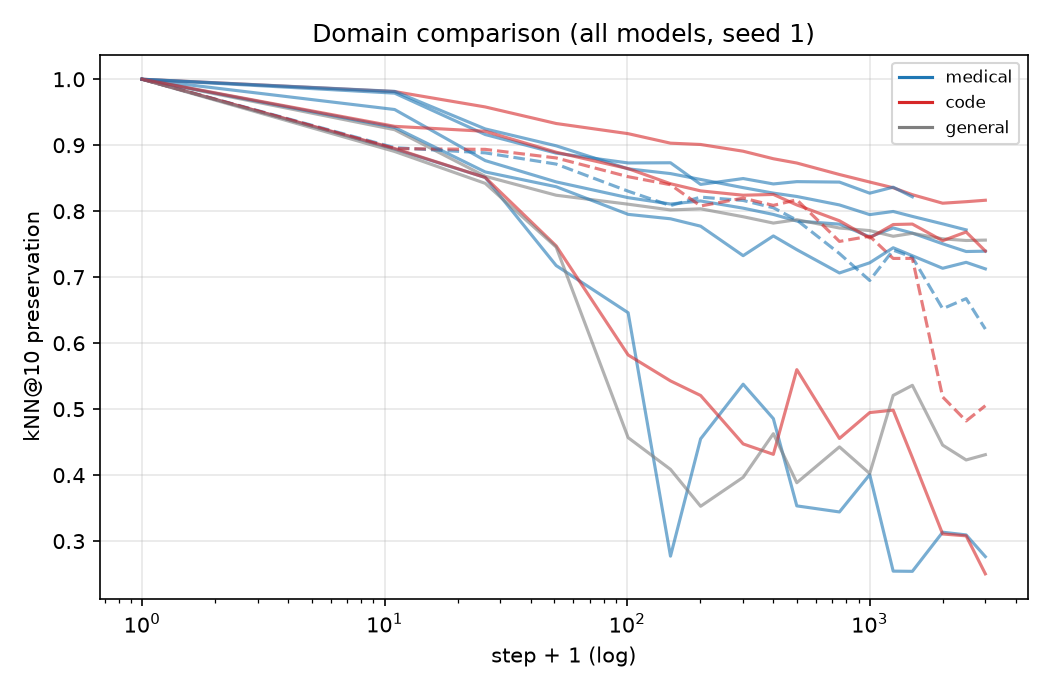
\includegraphics[width=0.6\linewidth]{figures/fig4_domain_comparison.png}
    \caption{\pres for all models (seed 1), coloured by fine-tuning domain. Among the stable runs at the top, code (red) usually lies above medical (blue). The low cluster is the diverging \pythiaS LoRA runs.}
    \label{fig:domain}
\end{figure}

\para{Software.} Python 3.12.12, torch 2.14.1, transformers 5.20.2, peft 0.21.2, numpy 2.5.4, scipy 1.18.1, pandas 3.1.0. No external APIs were used.
